\documentclass[a4paper,11pt,landscape,exos]{nsi} % COMPILE WITH DRAFT
\usepackage{hyperref}

\pagestyle{empty}
\setlength{\columnseprule}{0.5pt}
\setlength{\columnsep}{1cm}
\begin{document}

\begin{multicols}{2}
\classe{\terminale Comp}
\titre{\includegraphics[width=3cm]{CAN.png} Entrainement 7}
\maketitle


    Pour les questions \textbf{1.}, \textbf{2.} et \textbf{3.}, on donne les courbes de deux fonctions $f$ et $g$ :\\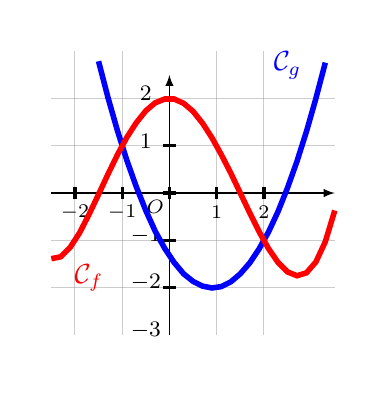
\begin{tikzpicture}[baseline,scale = 0.6]

        \tikzset{
          point/.style={
            thick,
            draw,
            cross out,
            inner sep=0pt,
            minimum width=5pt,
            minimum height=5pt,
          },
        }
        \clip (-3,-3.65) rectangle (4,3.5);
            \draw[color ={black},>=latex,->] (-2.5,0)--(3.5,0);
        \draw[color ={black},>=latex,->] (0,-3)--(0,2.5);
        \draw[color ={gray},opacity = 0.4] (-2.5,1)--(3.5,1);
        \draw[color ={gray},opacity = 0.4] (-2.5,-1)--(3.5,-1);
        \draw[color ={gray},opacity = 0.4] (-2.5,2)--(3.5,2);
        \draw[color ={gray},opacity = 0.4] (-2.5,-2)--(3.5,-2);
        \draw[color ={gray},opacity = 0.4] (1,-3)--(1,3);
        \draw[color ={gray},opacity = 0.4] (-1,-3)--(-1,3);
        \draw[color ={gray},opacity = 0.4] (2,-3)--(2,3);
        \draw[color ={gray},opacity = 0.4] (-2,-3)--(-2,3);
        \draw[color ={black},line width = 1.2] (0,-0.13)--(0,0.13);
        \draw[color ={black},line width = 1.2] (1,-0.13)--(1,0.13);
        \draw[color ={black},line width = 1.2] (-1,-0.13)--(-1,0.13);
        \draw[color ={black},line width = 1.2] (2,-0.13)--(2,0.13);
        \draw[color ={black},line width = 1.2] (-2,-0.13)--(-2,0.13);
        \draw[color ={black},line width = 1.2] (-0.13,0)--(0.13,0);
        \draw[color ={black},line width = 1.2] (-0.13,1)--(0.13,1);
        \draw[color ={black},line width = 1.2] (-0.13,-1)--(0.13,-1);
        \draw[color ={black},line width = 1.2] (-0.13,2)--(0.13,2);
        \draw[color ={black},line width = 1.2] (-0.13,-2)--(0.13,-2);
        \draw (1,-0.4) node[anchor = center, rotate=0] {\scriptsize \color{black}{$1$}};
        \draw (2,-0.4) node[anchor = center, rotate=0] {\scriptsize \color{black}{$2$}};
        \draw (-1,-0.4) node[anchor = center, rotate=0] {\scriptsize \color{black}{$-1$}};
        \draw (-2,-0.4) node[anchor = center, rotate=0] {\scriptsize \color{black}{$-2$}};
        \draw (-0.5,1.1) node[anchor = center, rotate=0] {\footnotesize \color{black}{$1$}};
        \draw (-0.5,2.1) node[anchor = center, rotate=0] {\footnotesize \color{black}{$2$}};
        \draw (-0.5,-0.9) node[anchor = center, rotate=0] {\footnotesize \color{black}{$-1$}};
        \draw (-0.5,-1.9) node[anchor = center, rotate=0] {\footnotesize \color{black}{$-2$}};
        \draw (-0.5,-2.9) node[anchor = center, rotate=0] {\footnotesize \color{black}{$-3$}};
        \draw (-0.3,-0.3) node[anchor = center, rotate=0] {\scriptsize \color{black}{$\text{O}$}};
        \draw (2.5,2.7) node[anchor = center, rotate=0] {\normalsize \color{blue}{$\mathcal{C}_g$}};
        \draw (-1.7,-1.8) node[anchor = center, rotate=0] {\normalsize \color{red}{$\mathcal{C}_f$}};
        \draw[color={blue},line width = 2] (-1.5,2.79)--(-1.3,2.02)--(-1.1,1.32)--(-0.9,0.69)--(-0.7,0.13)--(-0.5,-0.37)--(-0.3,-0.81)--(-0.1,-1.17)--(0.1,-1.47)--(0.3,-1.71)--(0.5,-1.87)--(0.7,-1.97)--(0.9,-2.01)--(1.1,-1.98)--(1.3,-1.88)--(1.5,-1.71)--(1.7,-1.48)--(1.9,-1.18)--(2.1,-0.82)--(2.3,-0.39)--(2.5,0.11)--(2.7,0.67)--(2.9,1.3)--(3.1,2)--(3.3,2.76);
        \draw[color={red},line width = 2] (-2.5,-1.39)--(-2.3,-1.35)--(-2.1,-1.15)--(-1.9,-0.84)--(-1.7,-0.45)--(-1.5,-0.03)--(-1.3,0.4)--(-1.1,0.81)--(-0.9,1.18)--(-0.7,1.49)--(-0.5,1.74)--(-0.3,1.91)--(-0.1,1.99)--(0.1,1.99)--(0.3,1.9)--(0.5,1.73)--(0.7,1.48)--(0.9,1.17)--(1.1,0.81)--(1.3,0.42)--(1.5,0)--(1.7,-0.42)--(1.9,-0.82)--(2.1,-1.18)--(2.3,-1.47)--(2.5,-1.67)--(2.7,-1.75)--(2.9,-1.69)--(3.1,-1.46)--(3.3,-1.03)--(3.5,-0.37);
    
    \end{tikzpicture} 
    \begin{enumerate}[itemsep=0.3cm]
        \item Image de $2$ par $f$
        \item Résoudre $f(x)>1$.
        \item Solutions de $f(x)=g(x)$
        \item $f(x)=x^2+x+1$\\$f(-4)=\ldots$
        \item $2$ stylos identiques coûtent $3$ €. 
            Quel est le prix de $3$ stylos ? \\$\ldots$ €
        \item Équation réduite de la droite $(AB)$.\\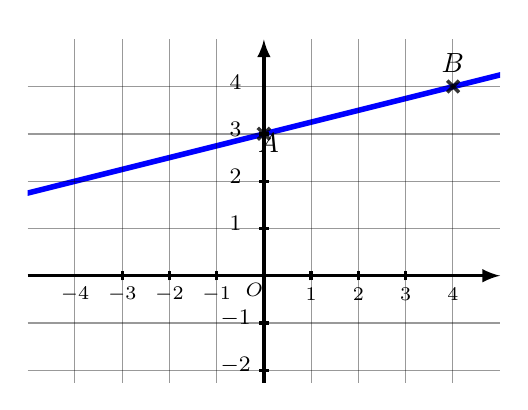
\begin{tikzpicture}[baseline,scale = 0.6]
    
            \tikzset{
                point/.style={
                  thick,
                  draw,
                  cross out,
                  inner sep=0pt,
                  minimum width=5pt,
                  minimum height=5pt,
                },
              }
              \clip (-5,-2.25) rectangle (5,5.25);
                  \draw[color={blue},line width = 2] (-48.54,-9.14)--(52.54,16.14);
              \draw[color ={black},line width = 1.2,>=latex,->] (-5,0)--(5,0);
              \draw[color ={black},line width = 1.2,>=latex,->] (0,-5)--(0,5);
              \draw[color ={black},opacity = 0.4] (-5,1)--(5,1);
              \draw[color ={black},opacity = 0.4] (-5,-1)--(5,-1);
              \draw[color ={black},opacity = 0.4] (-5,2)--(5,2);
              \draw[color ={black},opacity = 0.4] (-5,-2)--(5,-2);
              \draw[color ={black},opacity = 0.4] (-5,3)--(5,3);
              \draw[color ={black},opacity = 0.4] (-5,-3)--(5,-3);
              \draw[color ={black},opacity = 0.4] (-5,4)--(5,4);
              \draw[color ={black},opacity = 0.4] (-5,-4)--(5,-4);
              \draw[color ={black},opacity = 0.4] (1,-5)--(1,5);
              \draw[color ={black},opacity = 0.4] (-1,-5)--(-1,5);
              \draw[color ={black},opacity = 0.4] (2,-5)--(2,5);
              \draw[color ={black},opacity = 0.4] (-2,-5)--(-2,5);
              \draw[color ={black},opacity = 0.4] (3,-5)--(3,5);
              \draw[color ={black},opacity = 0.4] (-3,-5)--(-3,5);
              \draw[color ={black},opacity = 0.4] (4,-5)--(4,5);
              \draw[color ={black},opacity = 0.4] (-4,-5)--(-4,5);
              \draw[color ={black},line width = 1.2] (0,-0.1)--(0,0.1);
              \draw[color ={black},line width = 1.2] (1,-0.1)--(1,0.1);
              \draw[color ={black},line width = 1.2] (-1,-0.1)--(-1,0.1);
              \draw[color ={black},line width = 1.2] (2,-0.1)--(2,0.1);
              \draw[color ={black},line width = 1.2] (-2,-0.1)--(-2,0.1);
              \draw[color ={black},line width = 1.2] (3,-0.1)--(3,0.1);
              \draw[color ={black},line width = 1.2] (-3,-0.1)--(-3,0.1);
              \draw[color ={black},line width = 1.2] (-0.1,0)--(0.1,0);
              \draw[color ={black},line width = 1.2] (-0.1,1)--(0.1,1);
              \draw[color ={black},line width = 1.2] (-0.1,-1)--(0.1,-1);
              \draw[color ={black},line width = 1.2] (-0.1,2)--(0.1,2);
              \draw[color ={black},line width = 1.2] (-0.1,-2)--(0.1,-2);
              \draw[color ={black},line width = 1.2] (-0.1,3)--(0.1,3);
              \draw[color ={black},line width = 1.2] (-0.1,-3)--(0.1,-3);
              \draw (1,-0.4) node[anchor = center, rotate=0] {\scriptsize \color{black}{$1$}};
              \draw (2,-0.4) node[anchor = center, rotate=0] {\scriptsize \color{black}{$2$}};
              \draw (3,-0.4) node[anchor = center, rotate=0] {\scriptsize \color{black}{$3$}};
              \draw (4,-0.4) node[anchor = center, rotate=0] {\scriptsize \color{black}{$4$}};
              \draw (-1,-0.4) node[anchor = center, rotate=0] {\scriptsize \color{black}{$-1$}};
              \draw (-2,-0.4) node[anchor = center, rotate=0] {\scriptsize \color{black}{$-2$}};
              \draw (-3,-0.4) node[anchor = center, rotate=0] {\scriptsize \color{black}{$-3$}};
              \draw (-4,-0.4) node[anchor = center, rotate=0] {\scriptsize \color{black}{$-4$}};
              \draw (-0.6,1.1) node[anchor = center, rotate=0] {\footnotesize \color{black}{$1$}};
              \draw (-0.6,2.1) node[anchor = center, rotate=0] {\footnotesize \color{black}{$2$}};
              \draw (-0.6,3.1) node[anchor = center, rotate=0] {\footnotesize \color{black}{$3$}};
              \draw (-0.6,4.1) node[anchor = center, rotate=0] {\footnotesize \color{black}{$4$}};
              \draw (-0.6,-0.9) node[anchor = center, rotate=0] {\footnotesize \color{black}{$-1$}};
              \draw (-0.6,-1.9) node[anchor = center, rotate=0] {\footnotesize \color{black}{$-2$}};
              \draw (-0.6,-2.9) node[anchor = center, rotate=0] {\footnotesize \color{black}{$-3$}};
              \draw (-0.6,-3.9) node[anchor = center, rotate=0] {\footnotesize \color{black}{$-4$}};
              \draw[color ={black},line width = 1.25,opacity = 0.8] (-0.13,3.13)--(0.13,2.88);\draw[color ={black},line width = 1.25,opacity = 0.8] (-0.13,2.88)--(0.13,3.13);
              \draw (0.1,2.8) node[anchor = center, rotate=0] {\normalsize \color{black}{$A$}};
              \draw (4,4.5) node[anchor = center, rotate=0] {\normalsize \color{black}{$B$}};
              \draw[color ={black},line width = 1.25,opacity = 0.8] (3.88,4.13)--(4.13,3.88);\draw[color ={black},line width = 1.25,opacity = 0.8] (3.88,3.88)--(4.13,4.13);
              \draw (-0.2,-0.3) node[anchor = center, rotate=0] {\scriptsize \color{black}{$\text{O}$}};
          
          \end{tikzpicture}
	\item Multiplier une quantité par $0{,}65$ revient à la diminuer de : $\ldots\,\%$
	\item $(u_n)$ est une suite géométrique telle que $u_1=4$ et $u_2=-2$\\La raison de cette suite est :  $\ldots$
	
	\item Solution de l'équation $6x-3=9$

	
	\item $f(x)=x^3-2x^2-6\ ; \qquad$
    $f'(x)=$ $\ldots$
	
\end{enumerate}


\vfill\null



Score : \ldots\ldots / 10
\end{multicols}

\newpage

\begin{multicols}{2}
    \classe{\terminale Comp}
\titre{\includegraphics[width=3cm]{CAN.png} Corrigé 7}
\maketitle

\begin{enumerate}[]

\item L'image de $2$ se lit sur l'axe des ordonnées. \\
              On lit $f(2)={\color[HTML]{f15929}\boldsymbol{-1}}$. 
\item Les solutions de l'inéquation sont les abscisses des points de $\mathcal{C}_f$ qui se trouvent au-dessus de la droite horizontale d'équation $y=1$.\\
    $S={\color[HTML]{f15929}\boldsymbol{]-1\,;\,1[}}$ 
\item Les solutions sont les abscisses des points d'intersection entre les deux courbes :
   $S=\{{\color[HTML]{f15929}\boldsymbol{-1\,;\,2}}\}$. 
\item $f(-4)=\left(-4 \right)^2 -4 +1 = 13$\\
    On a donc $f(-4)={\color[HTML]{f15929}\boldsymbol{13}}$.
\item $2$ stylos coûtent $3$ €.\\
          $1$ stylo coûte  $1{,}50$ €.\\
          Ainsi,   $3$ stylos coûtent $3+ 1{,}50 ={\color[HTML]{f15929}\boldsymbol{4{,}50}}$ €.
\item Le coefficient directeur $m$ de la droite $(AB)$ est donné par :

Le coefficient directeur $m$ de la droite $(AB)$ est donné par :

\medskip

            $m=\dfrac{y_B-y_A}{x_B-x_A}=\dfrac{4-3}{4-0}=\dfrac{{\color{blue}\boldsymbol{1}}}{{\color{red}\boldsymbol{4}}}{\color[HTML]{f15929}\boldsymbol{}}$.

\medskip
L'ordonnée à l'origine est $b=f(0)=1$.\\
L'équation de la droite $(AB)$ est donc :
\begin{center}
    $\color[HTML]{f15929}\boldsymbol{y=\dfrac{1}{4}x+1}$.
\end{center}
\item On a $0{,}65=1-0{,}35$.\\
    Donc, diminuer une quantité de $0{,}65$ revient à la diminuer de $\color[HTML]{f15929}\boldsymbol{35\%}$.
\item La raison de la suite est donnée par :
\begin{center}
    $q=\dfrac{u_2}{u_1}=\dfrac{-2}{4}=\color[HTML]{f15929}\boldsymbol{-0{,}5}$.
\end{center}
\item \begin{tabbing}
    $6x-3=9\quad$ \= $\iff \quad 6x=9+3$ \\
    \> $\iff \quad 6x=12$\\
    \> $\iff \quad x=\dfrac{12}{6}$\\
    \> $\iff \quad x=2$.
\end{tabbing}
La solution de l'équation est donc $\color[HTML]{f15929}\boldsymbol{2}$.
\item \begin{tabbing}
    $f'(x)$ \= $=3x^2-2\times 2x-0$\\
    \> $=\color[HTML]{f15929}\boldsymbol{3x^2-4x}$
\end{tabbing}

\vfill\null

\end{enumerate}

\end{multicols}

\end{document}
